% Versuchsskript (Versuchsvorbereitung) MRT-Praktikum, LaTeX-Fassung.
% Übertragen aus der bisherigen PDF-Fassung (Google-Docs-Export, Stand 29.10.2026).
% Kompilieren aus diesem Ordner: latexmk -pdf Versuchsskript.tex
% Alternativ: pdflatex Versuchsskript.tex (zweimal).
% Alle Abbildungen liegen unter images/.
\documentclass[a4paper,11pt]{article}
\usepackage[T1]{fontenc}
\usepackage[utf8]{inputenc}
\usepackage[ngerman]{babel}
\usepackage{lmodern}
\usepackage[scaled=.92]{helvet}
\renewcommand{\familydefault}{\sfdefault}
\usepackage{microtype}
\usepackage[margin=25mm,top=22mm,bottom=25mm,headheight=14pt]{geometry}
\usepackage{graphicx,amsmath,amssymb}
\usepackage{xcolor}
\usepackage{enumitem,parskip,fancyhdr,lastpage,needspace}
\usepackage[explicit]{titlesec}
\usepackage[most]{tcolorbox}
\usepackage[font={small,it},labelfont={small,it},labelsep=colon,skip=6pt,justification=raggedright,singlelinecheck=false]{caption}
\usepackage[colorlinks=true,urlcolor=rwthblau,linkcolor=rwthblau,citecolor=rwthblau]{hyperref}
\graphicspath{{images/}}

% ---------------------------------------------------------------------------
% Interne Notizen des Betreuungsteams (Abschnitt 4) ein- oder ausblenden.
% \interntrue  : Notizen erscheinen als markierte Kästen (Betreuungsfassung).
% \internfalse : Studierendenfassung ohne Notizen (Standard).
\newif\ifintern
\internfalse
% ---------------------------------------------------------------------------

\definecolor{rwthblau}{HTML}{00549F}
\definecolor{titelgrau}{HTML}{666666}
\definecolor{dunkel}{HTML}{1F1F1F}
\definecolor{linie}{HTML}{888888}
\definecolor{warnrot}{HTML}{FF0000}

\hypersetup{
  pdftitle={Bildgebende Verfahren - Magnetresonanztomographie (MRT)},
  pdfsubject={Versuchsskript: Fett-Wasser-Trennung mit der Dixon-Methode am 1.5 Tesla MRT},
  pdfdisplaydoctitle=true}

\pagestyle{fancy}
\fancyhf{}
\fancyhead[L]{\small\color{titelgrau}Praktikum Medizintechnik\enspace|\enspace Magnetresonanztomographie}
\fancyhead[R]{\small\color{titelgrau}Versuchsskript}
\fancyfoot[R]{\small\thepage\,/\,\pageref*{LastPage}}
\renewcommand{\headrulewidth}{0.4pt}
\fancypagestyle{titel}{\fancyhf{}\renewcommand{\headrulewidth}{0pt}\fancyfoot[R]{\small\thepage\,/\,\pageref*{LastPage}}}

\setlength{\parindent}{0pt}
\setlength{\parskip}{6pt}
\setlength{\emergencystretch}{2em}
\setlist[itemize]{label=\textbullet,leftmargin=8mm,itemsep=1pt,parsep=0pt,topsep=0pt}
\setlist[enumerate]{leftmargin=8mm,itemsep=1pt,parsep=0pt,topsep=0pt}

% Überschriften wie im Original: Kapitel mit grauer Linie davor, Abschnitte kleiner.
\titleformat{\section}{\color{dunkel}\Large\bfseries}{}{0pt}
  {{\color{linie}\rule{\linewidth}{0.6pt}}\\[4mm]\thesection.\ #1}
\titleformat{name=\section,numberless}{\color{dunkel}\Large\bfseries}{}{0pt}
  {{\color{linie}\rule{\linewidth}{0.6pt}}\\[4mm]#1}
\titlespacing*{\section}{0pt}{8mm}{3mm}
\titleformat{\subsection}{\color{black}\large\bfseries}{}{0pt}{\thesubsection\ #1}
\titleformat{name=\subsection,numberless}{\color{black}\large\bfseries}{}{0pt}{#1}
\titlespacing*{\subsection}{0pt}{5mm}{1.5mm}

\newcommand{\lernziel}[1]{{\color{dunkel}\itshape Lernziel: #1\par}}
\newcommand{\absatzkopf}[1]{\par\vspace{2pt}\textbf{#1}\par\nopagebreak}
\newcommand{\pfeil}{$\rightarrow$}

\newtcolorbox{merke}{enhanced,frame hidden,colback=rwthblau!6,borderline west={2pt}{0pt}{rwthblau},
  arc=0pt,left=4mm,right=3mm,top=2mm,bottom=2mm,before skip=8pt,after skip=8pt,fontupper=\bfseries\color{titelgrau}}
\newtcolorbox{internbox}{enhanced,colback=orange!8,colframe=orange!70!black,boxrule=.4pt,arc=1mm,
  left=2mm,right=2mm,top=1mm,bottom=1mm,before skip=3pt,after skip=3pt,fontupper=\small,
  title={Notiz (intern)},fonttitle=\scriptsize\bfseries,coltitle=orange!40!black,colbacktitle=orange!20,
  attach boxed title to top left={xshift=2mm,yshift=-2mm},boxed title style={boxrule=0pt,arc=1mm}}
\newcommand{\intern}[1]{\ifintern\begin{internbox}#1\end{internbox}\fi}

% Mathematische Kurzschreibweisen
\newcommand{\Mxy}{M_{xy}}
\newcommand{\dphi}{\Delta\varphi}
\newcommand{\cs}{_{\mathit{cs}}}
\newcommand{\TE}{\mathit{TE}}
\newcommand{\IP}{_{\mathit{IP}}}
\newcommand{\OP}{_{\mathit{OP}}}
\newcommand{\unit}[1]{\,\mathrm{#1}}

\begin{document}
\thispagestyle{titel}

% ===================================================================== Titel
\pdfbookmark[0]{Titel}{titel}
\begin{flushright}

\includegraphics[width=125mm]{logo_lfb_rwth.png}
\end{flushright}
\vspace{10mm}
{\color{titelgrau}\large Praktikum Medizintechnik - Versuchsskript\par}
\vspace{3mm}
{\color{rwthblau}\fontsize{26}{31}\selectfont\bfseries Magnetresonanztomographie\par}
\vspace{2mm}
{\color{rwthblau}\fontsize{21}{27}\selectfont Fett-Wasser-Trennung mit der Dixon-\\Methode am 1.5 Tesla MRT\par}
\vspace{8mm}
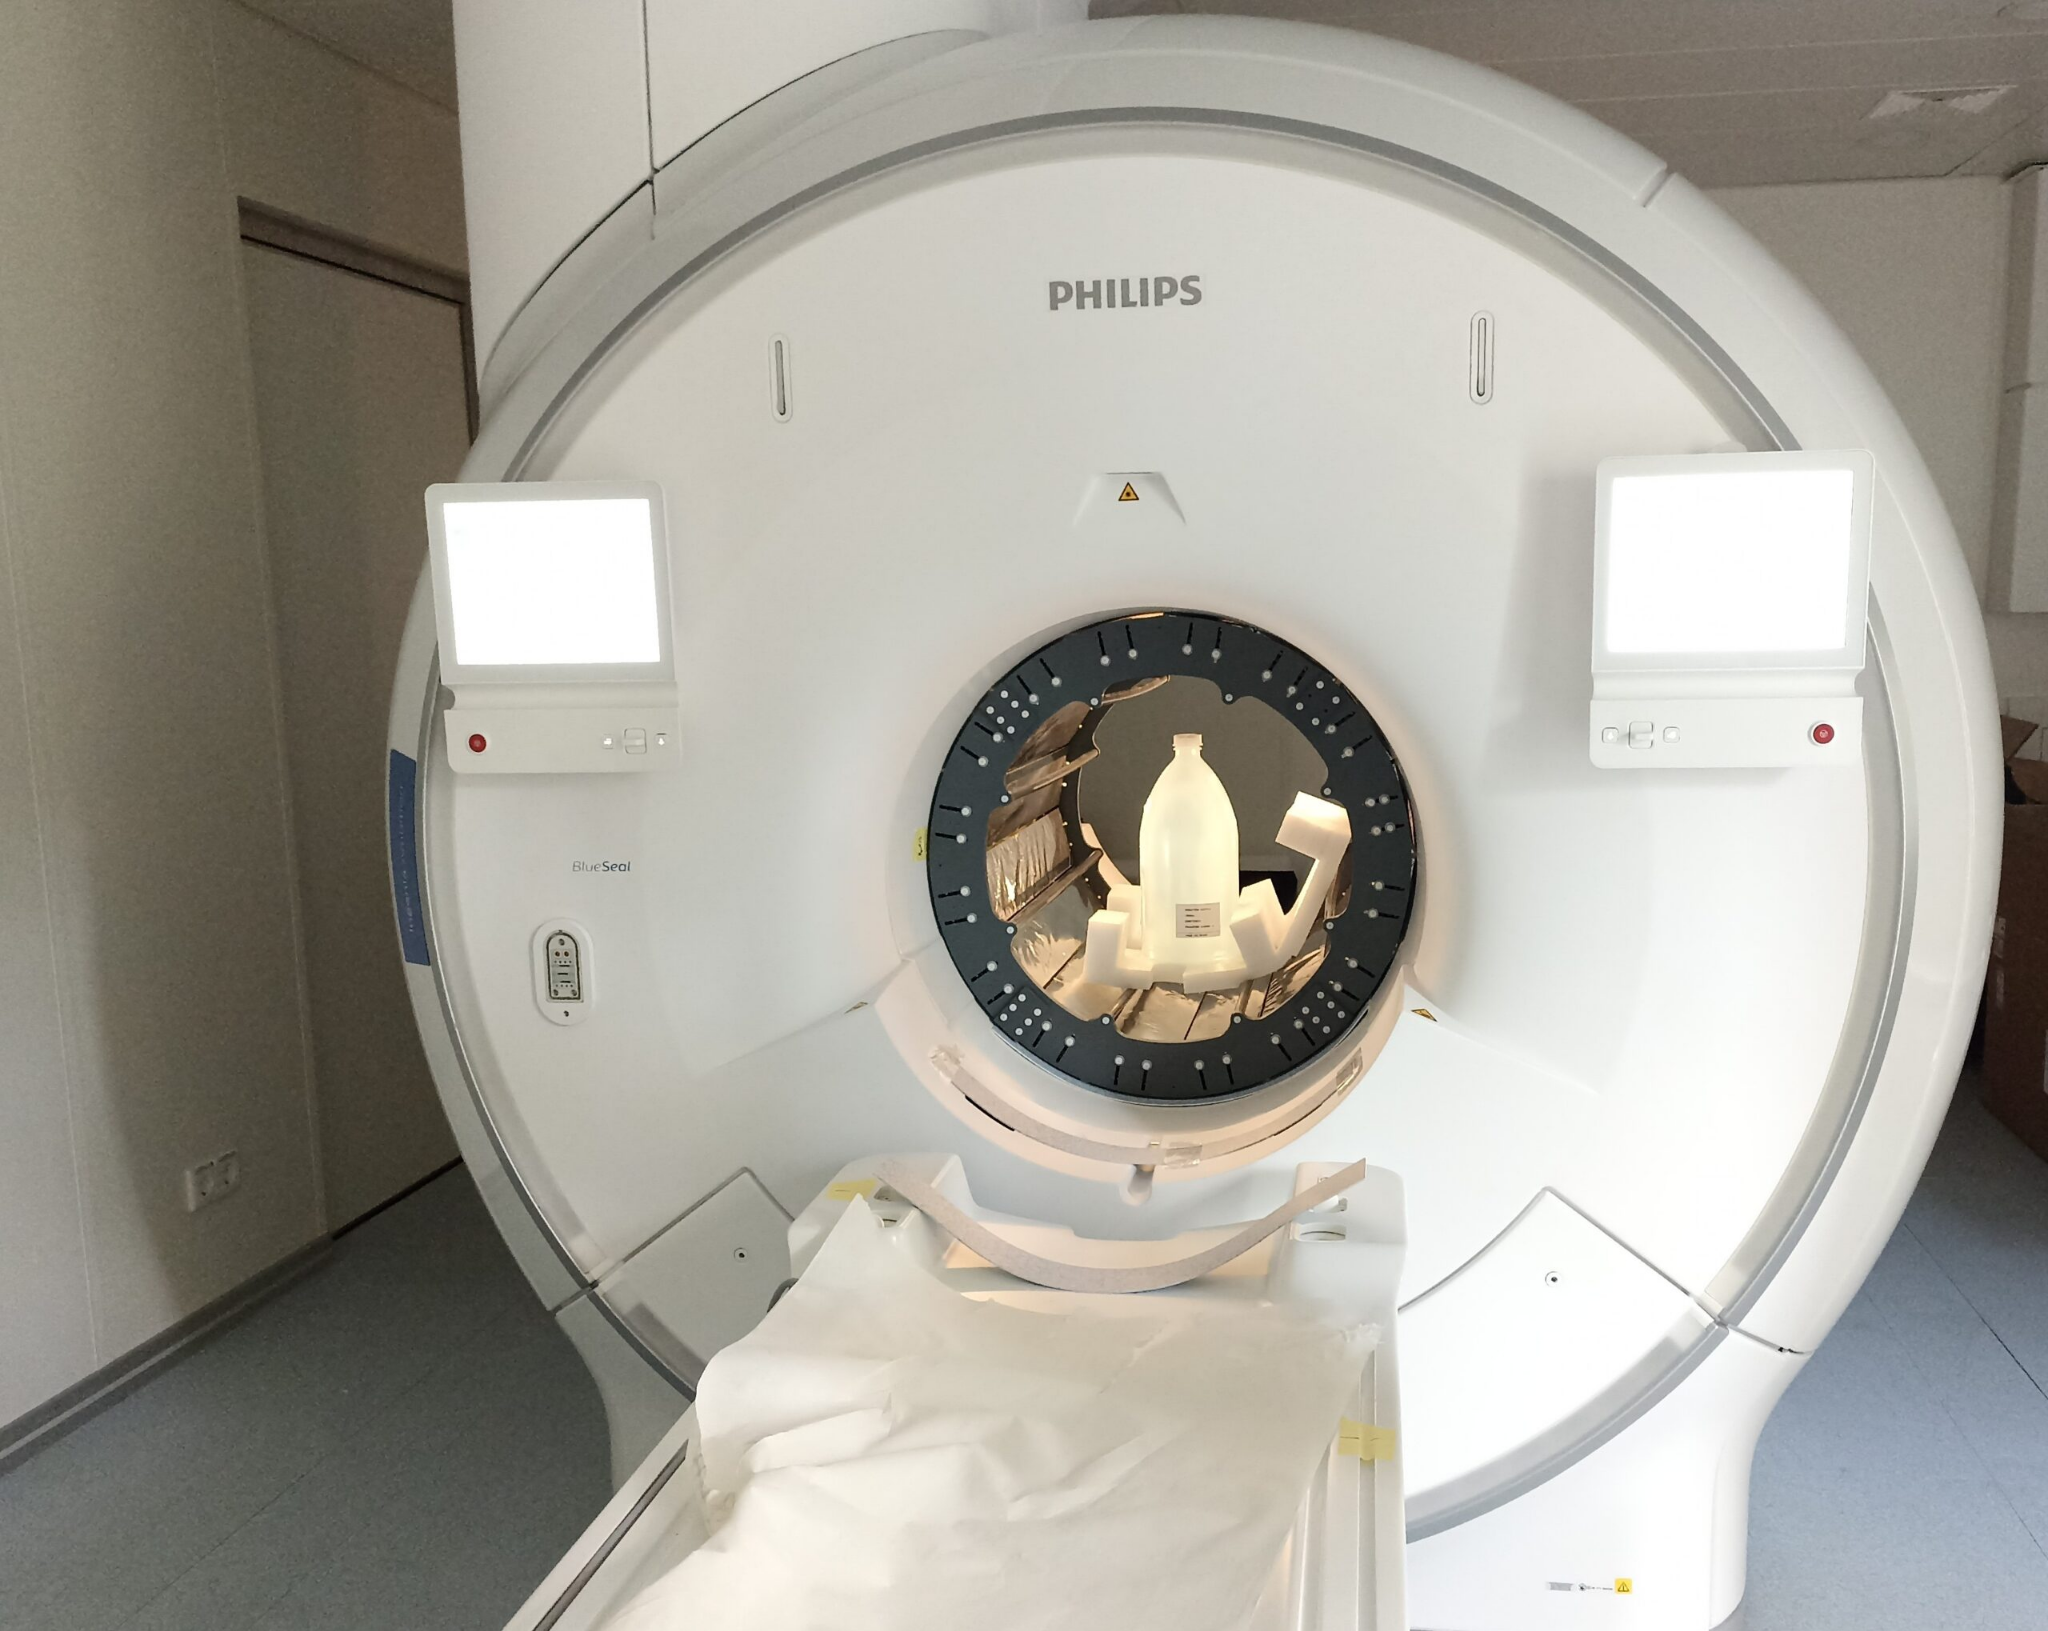
\includegraphics[width=88mm]{mrt_scanner.png}
\vspace{2mm}

% ===================================================================== 1
\section{Einleitung \& Klinische Motivation}\label{sec:einleitung}
\lernziel{Verstehen, was der Nutzen der MRT-Bildgebung ist und wozu die Fett-Wasser-Trennung (chemical shift-encoded MRT/Dixon-Technik) klinisch benötigt wird.}

\subsection{Nutzen der MRT-Bildgebung}
Die Magnetresonanztomographie (MRT) ist eine Bildgebungsmethode, die sich durch einen exzellenten Weichteilkontrast sowie durch das Fehlen ionisierender Strahlung auszeichnet.
Mittels verschiedener Arten von MRT-Sequenzen bzw.\ den daraus resultierenden Bildkontrasten können ganz unterschiedliche Fragestellungen beantwortet werden. Die verschiedenen Bildkontraste (man spricht in dem Zusammenhang auch von \glqq Gewichtungen\grqq) können anatomische, aber auch funktionelle Eigenschaften von Weichteilgeweben darstellen. Die Abwesenheit von ionisierender Strahlung macht die MRT im Vergleich zur CT viel schonender für die Patienten, da diese keiner Röntgenstrahlung ausgesetzt sind. Deshalb kann die MRT auch besonders gut für junge Patienten oder für Patienten, die viele Kontrolluntersuchungen benötigen, angewendet werden.

Der vorliegende MRT-Versuch befasst sich mit der Darstellung von Fett und Wasser im MRT. Die meisten Gewebe im Körper sind wässrige Gewebe, aber es gibt natürlich auch Fett: subkutanes (Unterhaut-), viszerales (Bauch-), perivaskuläres (um die Gefäße herum liegendes) Fettgewebe, oder das fetthaltige Knochenmark. Fett ist insofern ein besonderes Weichteilgewebe, da es eine leicht andere Resonanzfrequenz als wässrige Gewebe besitzt. Anhand der Wasser/Fett-Darstellung kann man nicht nur viel über die MRT-Bildgebung lernen. Sie ist tatsächlich auch in der klinischen MRT-Bildgebung sehr relevant.

\subsection{Wasser-Fett Darstellung in der Tumorbildgebung}
Ein wichtiges Anwendungsfeld für die Wasser/Fett-Bildgebung ist die Tumorbildgebung. Hier folgt auf die Erkennung einer sogenannten Raumforderung (\glqq ein Gewebe wächst dort, wo es nicht hingehört\grqq) deren Charakterisierung, um für den Patienten die bestmögliche Therapieoption zu finden. In diesem Kontext ist es sehr wichtig zu wissen, ob eine maligne (bösartige) oder eine benigne (gutartige) Raumforderung vorliegt. Um diese Einordnung vornehmen zu können, muss eine MRT-Untersuchung mehrere diagnostische Fragestellungen beantworten, zum Beispiel:
\begin{itemize}
\item Reichert die Raumforderung Kontrastmittel an?
\item Ist sie diffusionsgestört?
\item Besteht sie aus wässrigem Gewebe oder hat sie auch fettige Anteile?
\end{itemize}
Um zu wissen, ob eine Raumforderung fetthaltig ist, kann dieselbe Sequenz \glqq mit Fettunterdrückung\grqq\ wiederholt werden. Hierzu existieren verschiedene Techniken, die die unterschiedliche Resonanzfrequenz von fettigen und wässrigen Geweben ausnutzen. Wichtig sind in diesem Zusammenhang die spektrale Fettsuppression und die mittels chemischer Verschiebung kodierte MRT (engl.\ \glqq chemical shift encoded MRI\grqq, im Folgenden als CSE-MRT bezeichnet) zur Wasser-Fett-Trennung. Über die CSE-MRT kann häufig eine stabilere Fettsuppression erreicht werden als über eine spektrale Fettsuppression, weil sie robuster gegenüber Magnetfeld-Inhomogenitäten ist.

Also: die spektrale Fettsuppression unterdrückt das Fettsignal während der Akquisition, wohingegen die CSE-MRT die MRT-Daten in einem Postprocessing-Schritt in ein Wasser-Bild und ein Fett-Bild aufteilt.

Magnetfeldinhomogenitäten entstehen immer dann, wenn ein Patient/Objekt eine von Luft verschiedene Suszeptibilität hat. (Also eigentlich immer! In den meisten Fällen stört das die Bildgebung aber nicht relevant.) Anfällig für etwas stärkere Feldinhomogenitäten sind \glqq nicht zusammenhängende\grqq\ Anatomien mit vielen Luft-Gewebe-Grenzen, die zum Beispiel bei der Brustbildgebung (Lunge), der simultanen Bildgebung beider Beine, oder im Gastrointestinaltrakt auftreten können. Besonders starke Magnetfeldinhomogenitäten können in der Nähe von metallischem Fremdmaterial (z.\,B.\ künstliche Kniegelenke, künstliche Hüftgelenke) vorhanden sein. Hier versagen spektrale Fettsuppressionstechniken häufig völlig.

\begin{merke}
CSE-MRT-Sequenzen tragen in der MRT-Welt übrigens auch den Namen \glqq Dixon\grqq-Sequenzen, nach ihrem Erfinder W.~Thomas Dixon, der dazu 1984 eine grundlegende wissenschaftliche Arbeit veröffentlicht hat.
\end{merke}

\subsection{Fettquantifizierung in der Leberbildgebung}
Ein weiteres Anwendungsbeispiel für die CSE-MRT aus dem klinischen Alltag ist die Leberverfettung, die im Zusammenhang mit der MASLD-Erkrankung (\glqq metabolische Dysfunktion-assoziierte steatotische Lebererkrankung\grqq) auftritt. Eine Leberverfettung kann die erste Stufe einer ganzen Erkrankungs-Kaskade darstellen, die Leberzirrhose, Leberversagen und hepatozelluläre Karzinome bedingen kann. Sie stellt auch einen Risikofaktor für das metabolische Syndrom, Typ-2-Diabetes und kardiovaskuläre Mortalität dar. Die Therapie der Steatosis hepatis umfasst in der Regel eine Kombination aus Lebensstiländerungen und medikamentöser Behandlung. Häufig bleibt eine Leberverfettung bzw.\ MASLD allerdings leider lange unerkannt, zumindest im Frühstadium. Eine frühzeitige Diagnose und Behandlung sind wegen der möglichen Folgen jedoch entscheidend. Der Fettgehalt der Leber wurde traditionell über eine Biopsie festgestellt. Dies ist allerdings sehr invasiv, und außerdem kann so nur ein lokaler Fettgehalt bestimmt werden. Auch die MRT-Bildgebung kann eine Leberverfettung diagnostizieren. Dazu reicht es allerdings nicht, das reine Vorhandensein von Fett zu bejahen oder zu verneinen wie vielleicht bei der Tumorcharakterisierung. Stattdessen muss der genaue Fettgehalt des Organs quantifiziert werden, genauer gesagt, die sogenannte \glqq Proton Density Fat Fraction\grqq\ (PDFF). Dies kann CSE-MRT leisten, und zwar auf nicht invasive Weise! Moderne Sequenzen zur Fettquantifizierung erfassen dabei die PDFF über die ganze Leber in einem einzigen Atem-Anhalter des Patienten. Abbildung~\ref{fig:pdff} zeigt beispielhaft mittels CSE-MRT gewonnene PDFF-Karten der Leber für verschiedene Grade an Leberverfettung. [Starekova 2021]

\begin{figure}[htbp]
\centering
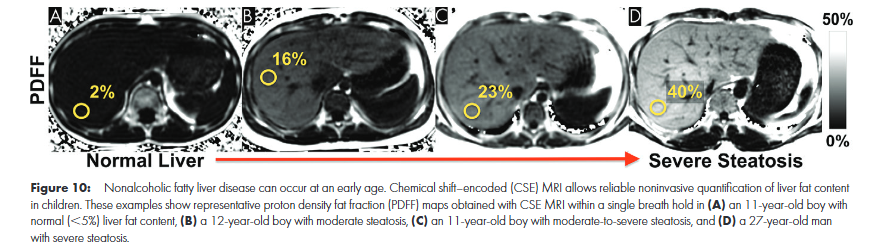
\includegraphics[width=\linewidth]{pdff_leber_starekova.png}
\caption{PDFF-Karten für unterschiedliche Grade an Leberverfettung, die mittels CSE-MRT gewonnen wurden. (aus Starekova et al.)}
\label{fig:pdff}
\end{figure}

\subsection{Ziel des Praktikums}
In diesem Praktikum sollen Sie die Grundlagen der Wasser-Fett-Trennung mittels CSE-MRT verstehen und anwenden. Dazu nehmen Sie an einem klinischen MRT-Gerät selbst geeignete Sequenzen auf und errechnen daraus mittels eines Python-Skriptes selbst Wasser- und Fettbilder.

% ===================================================================== 2
\section{Physikalische Grundlagen der MRT}\label{sec:grundlagen}
{\color{dunkel}Lernziel: Ein Basisverständnis der Signalentstehung und des MRT-Bildkontrastes gewinnen.\\
Hinweis für E-Techniker: Betrachten Sie das MRT als ein Übertragungssystem, das Antwortsignale auf HF-Anregung misst.\par}

\subsection{Der Kernspin und das \texorpdfstring{$B_0$}{B0}-Feld}
Atomkerne mit ungerader Nukleonenzahl (wie Wasserstoff $^{1}\mathrm{H}$) besitzen einen Eigendrehimpuls (Spin) und somit ein magnetisches Moment. Ohne äußeres Feld sind die magnetischen Momente chaotisch im Raum orientiert. In Summe verursachen sie also keine messbare Nettomagnetisierung.

Im starken Magnetfeld $B_0$ (in unserem Labor: 1.5 Tesla) richten sich die magnetischen Momente parallel oder antiparallel zum $B_0$-Feld aus. Da bei Raumtemperatur etwas mehr Spins in parallele Richtung zeigen als entgegengesetzt zum Feld, entsteht eine Netto-Magnetisierung $M_z$, die parallel zu $B_0$ ausgerichtet ist.

\needspace{6\baselineskip}
Die einzelnen magnetischen Momente präzedieren (kreiseln) um die Feldlinien mit der Larmor-Frequenz $\omega_0$:
\[
\omega_0 = \gamma \cdot B_0
\]
\begin{itemize}
\item $\gamma$: Gyromagnetisches Verhältnis (für Wasserstoff ca.\ $42.58\unit{MHz/T}$).
\item Bei 3 Tesla entspricht dies ca.\ $127.7\unit{MHz}$ (UKW-Radiobereich).
\end{itemize}

\emph{Anmerkung:} Im Gleichgewichtszustand (\glqq $B_0$-Feld an, aber ansonsten passiert nichts\grqq) \glqq sieht\grqq\ man die Präzession der einzelnen magnetischen Momente nicht, da diese im Allgemeinen nicht in Phase präzedieren. Die Nettomagnetisierung hat dann also keine $x$- oder $y$-Komponenten. Dies ändert sich erst, wenn die magnetischen Momente kohärent aus der Richtung des $B_0$-Feldes ausgelenkt werden (s.\ Abschnitt~\ref{sec:anregung}, Anregung).

Wir definieren die $B_0$-Richtung als die $z$-Achse eines Koordinatensystems. Die $xy$-Ebene des Koordinatensystems bezeichnen wir als die transversale Ebene. Betrachten wir das Verhalten der Magnetisierung als einen zeitabhängigen Vektor in diesem Koordinatensystem, sprechen wir von \glqq longitudinaler Magnetisierung\grqq\ ($M_z(t)$) und \glqq transversaler Magnetisierung\grqq\ ($\Mxy(t)$).

Aufgrund der Präzession bietet es sich an, für die Beschreibung der transversalen Magnetisierung eine Darstellung in Polarkoordinaten mit Magnitude und Phase zu verwenden. Durch Anregung und Relaxation kann longitudinale Magnetisierung in transversale Magnetisierung umgewandelt werden und andersherum.

\subsection{Anregung und Relaxation (T1 \& T2)}\label{sec:anregung}
Wird ein HF-Impuls (Hochfrequenz) mit genau der Larmor-Frequenz in das Gewebe gesendet, passieren zwei Dinge.

\textbf{Resonanz:} Die Magnetisierung kippt, solange der HF-Puls eingestrahlt wird, in Richtung der Transversalebene. Dort entsteht also eine transversale Magnetisierungskomponente $\Mxy$, die nach der Anregung mit der Frequenz $\omega_0$ um die $z$-Achse präzediert. Jetzt können wir mithilfe einer Empfangsspule, die wir in die Nähe der Probe/des Gewebes bringen, ein Signal messen. $\Mxy$ stellt einen sich zeitlich schnell verändernden magnetischen Fluss durch die Querschnittsfläche der Spule dar. Aufgrund der elektromagnetischen Induktion entsteht in der Spule also eine elektrische Spannung. Das gemessene Signal ist komplex; das heißt, der MRT-Scanner misst sowohl die Magnitude als auch die Phase von $\Mxy$. In der Klinik werden hauptsächlich Magnitudenbilder verwendet. Die Phase kann allerdings viele zusätzliche Informationen kodieren. Je nachdem, wie lange der HF-Puls eingestrahlt wird und je nach seiner Amplitude wird die Magnetisierung unterschiedlich weit in die transversale Ebene ausgelenkt. Man spricht in diesem Zusammenhang auch vom \glqq Flipwinkel\grqq, den man für jede MRT-Sequenz einstellen kann. Bei einem Flipwinkel von 90° wird die Magnetisierung vollständig in die transversale Ebene gekippt. Bei kleineren Flipwinkeln entstehen sowohl transversale als auch longitudinale Magnetisierungsanteile. Wichtig zu beachten ist: ohne Anregung kein MRT-Bild, da das MRT-Signal immer durch die transversale Magnetisierung $\Mxy$ gegeben ist!

\textbf{Relaxation:} Nach dem Abschalten des Pulses kehrt das System ins Gleichgewicht zurück.
\begin{enumerate}
\item \textbf{T1-Relaxation (Longitudinale Relaxation):} Wie schnell baut sich $M_z$ wieder auf? Die T1-Relaxation können Sie sich als ein \glqq Zurück-Spiralen\grqq\ (d.\,h., gleichzeitiges Präzedieren und wieder zurück in Richtung des $B_0$-Feldes Wandern) der Magnetisierung vorstellen. Betrachtet man nur die longitudinale Komponente der Magnetisierung, so folgt diese einer exponentiellen Wiederannäherung an ihren Ausgangswert $M_0$:
\[
M_z(t) = M_0 \cdot \bigl(1 - e^{-t/T_1}\bigr)
\]
Wie schnell die Wiederannäherung vonstatten geht, wird durch die T1-Relaxationszeit des Gewebes bestimmt. Diese Formel gilt für einen Flipwinkel von 90°, wir wollen an der Stelle nicht weiter ins Detail gehen.
\item \textbf{T2-Relaxation (Transversale Relaxation):} Wie schnell zerfällt das Signal $\Mxy$ durch Spin-Spin-Wechselwirkungen? Die T2-Relaxation können Sie sich als ein Dephasieren (\glqq Auseinander-Fächern\grqq) der einzelnen magnetischen Momente innerhalb der transversalen Ebene vorstellen - einige präzedieren etwas schneller, andere etwas langsamer. Das ist durch Interaktionsprozesse der magnetischen Momente untereinander bedingt. Hierdurch nimmt $\Mxy$, also die Summe über die einzelnen Momente, mit der Zeit ab. Diese Abnahme erfolgt ebenfalls exponentiell.
\[
\Mxy(t) = M_0 \cdot e^{-t/T_2}
\]
Hier bestimmt die T2-Relaxationszeit des Gewebes, wie schnell das Dephasieren passiert (auch hier ist wieder die Formel für eine 90° Anregung angegeben).
\end{enumerate}

Unterschiedliche Gewebe haben unterschiedliche Relaxationszeiten T1 und T2. Diese Unterschiede bilden die Basis für den Bildkontrast in MRT-Bildern. Wie genau jedes Gewebe auf einem MRT-Bild aussieht, also mit welchem Grauwert es zur Darstellung kommt, hängt zum einen von der verwendeten MRT-Sequenz und zum anderen von den genauen Einstellungen der Sequenzparameter ab. (Wie ist die zeitliche Abfolge von Anregungen und Signalmessungen? Welcher Flipwinkel wurde eingestellt?) Es gibt Sequenzen, für welche die T1-Relaxation den Bildkontrast dominiert (T1-gewichtete Sequenzen), und Sequenzen, für welche die T2-Relaxation den Bildkontrast dominiert (T2-gewichtete Sequenzen). Die meisten MRT-Sequenzen produzieren \glqq qualitative\grqq\ Bilder, auf denen die Gewebe unterschiedliche Grauwerte haben, aber der Grauwert selbst keine physikalische Bedeutung hat. (Das ist in der CT-Bildgebung anders - dort stellt der Grauwert die Hounsfield-Unit dar, von der man direkt auf den Schwächungskoeffizienten des Gewebes zurückrechnen kann.) Es ist auch in der MRT-Bildgebung möglich, mittels spezieller Sequenzen die Gewebeparameter selbst zu vermessen. Dann sprechen wir von \glqq quantitativen\grqq\ MRT-Sequenzen. Neben den Relaxationszeiten kann man mit solchen quantitativen MRT-Sequenzen zum Beispiel auch den Diffusionskoeffizienten eines Gewebes oder eben die PDFF (Fettgehalt) eines Gewebes untersuchen.

\subsection{Ortskodierung: Der k-Raum}
{\color{dunkel}\itshape Das Verständnis der Ortskodierung ist für dieses Praktikum nicht relevant. Daher reißen wir diese hier nur ganz kurz an.\par}

Wie wird aus dem Summensignal ein Bild? Wir nutzen Gradientenspulen, die das Magnetfeld linear über den Raum ändern ($B(x) = B_0 + G_x \cdot x$). Dadurch ändert sich die Resonanzfrequenz ortsabhängig.
\begin{itemize}
\item Für E-Techniker: Das MRT misst nicht das Bild direkt, sondern dessen \textbf{2D-Fourier-Transformation}. Diese Rohdaten nennen wir \textbf{k-Raum}.
\item Die Bildrekonstruktion ist (vereinfacht) eine inverse 2D-FFT:
\[
\mathrm{Bild}(x, y) = \mathcal{F}^{-1}\bigl\{k(k_x, k_y)\bigr\}
\]
\end{itemize}

\subsection{Wichtige Sequenzparameter}
Um ein MRT-Bild aufzunehmen und somit den k-Raum zu füllen, wird sehr oft hintereinander das Gewebe durch Einstrahlen eines HF-Pulses angeregt und im Folgenden jeweils die präzedierende transversale Magnetisierung $\Mxy$ gemessen. Zwei Sequenzparameter sind besonders wichtig, um den zeitlichen Ablauf einer MRT-Sequenz zu definieren.
\begin{itemize}
\item \textbf{Echozeit (TE):} Zeit zwischen Anregung (Senden des HF-Pulses) und Messung des MRT-Signals ($\Mxy$)
\item \textbf{Repetitionszeit (TR):} Zeit zwischen zwei aufeinanderfolgenden HF-Anregungen
\end{itemize}
Die TE und die TR bestimmen, wie viel Einfluss die T2- und die T1-Relaxation auf den Bildkontrast nehmen, oder anders formuliert, wie stark T2- oder T1-gewichtet das aufgenommene Bild sein wird:
\begin{itemize}
\item Je kürzer die TE ist, desto weniger Einfluss hat die T2-Relaxationszeit auf den Bildkontrast, da bei einer kurzen TE kein Gewebe genug \glqq Zeit hat\grqq, seine $xy$-Magnetisierung in der transversalen Ebene auseinander fächern bzw.\ dephasieren zu lassen.
\item Je länger die TR ist, desto weniger Einfluss hat die T1-Relaxationszeit auf den Bildkontrast, da bei einer langen TR alle Gewebe genug Zeit haben, die Magnetisierung wieder zum \glqq Ausgangspunkt\grqq\ zu bringen, d.\,h., parallel zu $B_0$.
\end{itemize}
Das Zustandekommen verschiedener Gewichtungen ist grundsätzlich sehr interessant, aber für den Praktikumsversuch erstmal nicht weiter relevant.

Die Echozeit hat aber noch einen anderen wichtigen Einfluss auf das MRT-Signal - sie bestimmt nämlich die Phase des gemessenen MRT-Signals. Das ist für den Versuch zur Wasser-Fett-Trennung sehr wichtig!

Je länger die Echozeit ist, desto länger präzediert $\Mxy$ - ergo, desto größer wird die akkumulierte Phase $\varphi$ des MRT-Signals:
\[
\varphi = \omega \cdot t = \gamma \cdot B \cdot t.
\]
Es ist zu beachten, dass die Phase $2\pi$-periodisch ist. Bei \glqq langen\grqq\ TEs kann es also durchaus vorkommen, dass die Phase von $\Mxy$ mehrere Male die vollen $2\pi$ durchläuft, bevor das MRT-Signal, also $\Mxy$, gemessen wird.

% ===================================================================== 3
\section{Die DIXON-Methode: Fett-Wasser-Trennung}\label{sec:dixon}
\lernziel{Den \glqq Chemical Shift\grqq-Effekt verstehen und mathematisch nutzen.}

\subsection{Der Chemical Shift (Chemische Verschiebung)}
Obwohl Fett- und Wassermoleküle beide Wasserstoffkerne enthalten, ist deren Elektronenumgebung unterschiedlich. Die Elektronenwolke schirmt das $B_0$-Feld leicht ab.
\begin{itemize}
\item Fett-Protonen \glqq sehen\grqq\ ein geringeres Feld als Wasser-Protonen.
\item Daher präzedieren sie etwas langsamer.
\item Der Frequenzunterschied $\Delta f$ beträgt ca.\ 3.5\,ppm. Entsprechend ist der chemical shift (cs) bei 1.5 Tesla: $\Delta f\cs \approx 220\unit{Hz}$.
\end{itemize}

\subsection{In-Phase und Out-of-Phase (Vektormodell)}
Stellen Sie sich Wasser ($M_{xy,W}$) und Fett ($M_{xy,F}$) als zwei rotierende Zeiger im komplexen Raum vor (im rotierenden Referenzsystem), mit Amplituden $W$ und $F$ und den Phasen $\varphi_W$ und $\varphi_F$. Da Fett eine niedrigere Resonanzfrequenz hat als Wasser, also langsamer präzediert, baut sich über die Zeit zwischen Anregung und Messung (Echo Time, TE) eine Phasendifferenz $\dphi\cs$ auf:
\[
\dphi\cs(\TE) = 2\pi \cdot \Delta f\cs \cdot \TE
\]
\begin{itemize}
\item \textbf{In-Phase (IP):} Für $\dphi\cs = 0, 2\pi, 4\pi, \ldots$ zeigen beide Zeiger in dieselbe Richtung. Das Summensignal ist maximal (Abbildung~\ref{fig:zeiger}a):
\[
M_{xy,\mathit{IP}} = W + F
\]
\item \textbf{Out-of-Phase (OP):} Für $\dphi\cs = \pi, 3\pi, 5\pi, \ldots$ zeigen die Zeiger in entgegengesetzte Richtungen. Das Summensignal ist minimal (Abbildung~\ref{fig:zeiger}b):
\[
M_{xy,\mathit{OP}} = \lvert W - F \rvert
\]
\end{itemize}
Abbildung~\ref{fig:zeiger}c stellt die vektorielle Addition von Wasser- und Fettsignal für den allgemeinen Fall dar.

\begin{figure}[htbp]
\centering
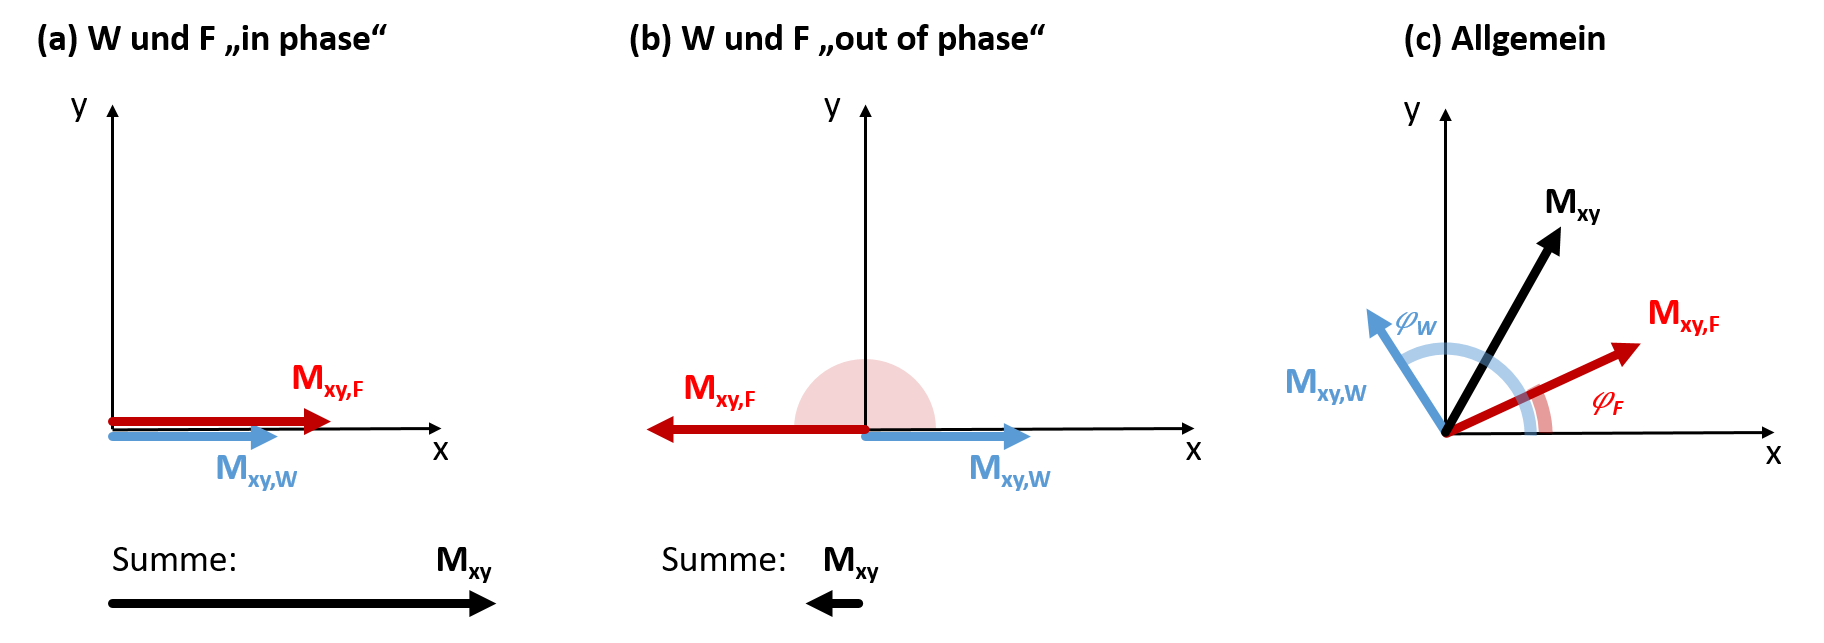
\includegraphics[width=\linewidth]{dixon_zeigerdiagramm.png}
\caption{Das gemessene MRT-Signal $\Mxy$ entsteht aus der Summe des Wasser-Signals und des Fettsignals durch vektorielle Addition. (a) zeigt eine Situation, in der die transversalen Magnetisierungen von Wasser und Fett in Phase sind. Dies ist zum Beispiel direkt nach der Anregung der Fall. Die beiden Signalanteile addieren sich konstruktiv. (b) zeigt eine Situation, in der die transversalen Magnetisierungen von Wasser und Fett genau gegenphasig sind. Das Summensignal ist gegenüber den Einzelsignalen reduziert. Bei anderen Phasendifferenzen liegt die Magnitude des Summensignals zwischen den beiden hier dargestellten Situationen.}
\label{fig:zeiger}
\end{figure}

\subsection{Rolle von Magnetfeldinhomogenitäten}
Sie wissen nun, dass die Stärke des $B_0$-Feldes über die Resonanzfrequenz bestimmt, wie viel Phase eine transversale Magnetisierung über die Zeit TE aufsammelt ($\varphi = \omega_0 \cdot \TE$). Außerdem wissen Sie, dass die chemische Natur eines Stoffes (Fett oder Wasser) bestimmt, ob diese Phase aufgrund der chemischen Verschiebung abweicht.

Es gibt allerdings noch einen weiteren Einfluss auf die Phase: die bereits erwähnten Magnetfeldinhomogenitäten. Wenn an einem Ort im Scanner eine von null verschiedene Suszeptibilität vorliegt, weicht das Magnetfeld dort lokal vom $B_0$-Feld ab. Die lokale Resonanzfrequenz $\omega$ unterscheidet sich dann von der erwarteten Larmorfrequenz $\omega_0$. Das führt ebenfalls zu einer Abweichung der lokalen Phase von der Phase, die allein aufgrund des $B_0$-Feldes zu erwarten wäre:
\[
\dphi(\TE) = \Delta\omega \cdot \TE
\]
Wasser- und Fettmagnetisierung sind dem Einfluss der Feldinhomogenitäten gleichermaßen ausgesetzt. Es gilt also:
\begin{align*}
\dphi_W &= \dphi\\
\dphi_F &= \dphi + \dphi\cs
\end{align*}
Unter Berücksichtigung der lokalen Magnetfeldinhomogenität und der chemischen Verschiebung von Fett erhält man zum Messzeitpunkt TE also das Summensignal:
\[
\Mxy(x, y, \TE) = \Bigl(W(x, y) + F(x, y) \cdot e^{i\dphi\cs(\TE)}\Bigr) \cdot e^{i\dphi(\TE)}
\]

\subsection{Die 2-Punkt-Dixon-Lösung}
Nehmen wir zwei Bilder auf, ein Bild $S_1$ zum Zeitpunkt $\TE\IP$ und ein Bild $S_2$ zum Zeitpunkt $\TE\OP$, erhalten wir ein Gleichungssystem. Für den einfachen Fall, also ohne $B_0$-Inhomogenitäten und unter Vernachlässigung von Relaxationsprozessen, gilt:
\begin{align*}
W &= \frac{\lvert S_1 + S_2 \rvert}{2}\\[2pt]
F &= \frac{\lvert S_1 - S_2 \rvert}{2}
\end{align*}
Dieser einfache Ansatz funktioniert allerdings nur, wenn keine oder nur sehr geringe Magnetfeldinhomogenitäten vorliegen. Andernfalls enthalten die berechneten Bilder im Allgemeinen Mischungen aus Wasser- und Fettsignal.

\subsection{Die 3-Punkt-Dixon-Lösung}
Die Trennung in Wasser- und Fettsignal wird robuster, wenn man den Einfluss der Hintergrundphase vorher herausrechnet. Das gelingt zum Beispiel, indem man zu einem dritten Messzeitpunkt erneut ein In-Phase-Bild aufnimmt, also ein Bild $S_3$ zum Zeitpunkt $\TE_{2\times\mathit{IP}}$. Über einen Vergleich der beiden In-Phase-Bilder lässt sich dann die Hintergrund-Feldinhomogenität in jedem Voxel berechnen:
\[
\dphi(x, y) = \frac{1}{2}\,\arg\Bigl(S_3(x, y) \cdot S_1^{*}(x, y)\Bigr)
\]
Dabei ist $S_1^{*}$ das komplex konjugierte Bild zu $S_1$. Damit können die Bilder $S_1$ bis $S_3$ um die Hintergrund-Feldinhomogenität korrigiert werden:
\begin{align*}
W &= \frac{1}{2}\left[\frac{1}{2}\Bigl(S_1 + S_3\,e^{-2i\dphi}\Bigr) + S_2\,e^{-i\dphi}\right]\\
F &= \frac{1}{2}\left[\frac{1}{2}\Bigl(S_1 + S_3\,e^{-2i\dphi}\Bigr) - S_2\,e^{-i\dphi}\right]
\end{align*}
Ein praktisches Problem ist das sogenannte \emph{Phase Wrapping}: Die Phase ist nur auf einem Intervall der Länge $2\pi$ definiert. Werden die Feldinhomogenität oder die Echozeit so groß, dass die Phase dieses Intervall überschreitet, treten in $\dphi$ Sprünge auf. Diese müssen mit einem \emph{Phase-Unwrapping}-Algorithmus korrigiert werden, bevor die Wasser-Fett-Trennung korrekt durchgeführt werden kann.

{\color{dunkel}Weitere Infos unter Ma, Dixon techniques for water and fat imaging, Journal of Magnetic Resonance Imaging 2008; 28:543--558.\par}

\subsection{Ausblick}
Die in-phase oder out-of-phase Zeitpunkte bieten eine analytische Lösung des Wasser-Fett-Separationsproblems, jedoch sind sie im Hinblick auf das Signal-Rausch-Verhältnis nicht ideal. \glqq Moderne\grqq\ Wasser-Fett-Separations-Algorithmen basieren zumeist auf iterativen Rekonstruktionen und nutzen mehrere, enger zusammenliegende Echozeiten. Dadurch können sie auch noch auf weitere \glqq confounding effects\grqq\ korrigieren.

% ===================================================================== 4
\section{Ablaufplan des Praktikums (Präsenz)}\label{sec:ablauf}
{\color{linie}\rule{\linewidth}{0.6pt}}\par
{\color{warnrot}\itshape\large\textbf{Hinweis:} Dieser Ablaufplan hat den Stand vom 29.10.2026. Bis zum 03.11.2026 kann es noch Änderungen geben. Danach gilt die finale Version, die wir rechtzeitig im Moodle Lernraum bereitstellen.\par}
{\color{linie}\rule{\linewidth}{0.6pt}}\par

\subsection*{Teil 1: Briefing \& Sicherheitsunterweisung (30 Min)}
\absatzkopf{Briefing:}
\begin{itemize}
\item Welcoming \& Ablauf
\item Refresher - MRT-Grundlagen.
\item Deep-Dive - Die Dixon-Methode und -Algebra.
\end{itemize}

\absatzkopf{Kurze Sicherheitsunterweisung:}
\begin{list}{}{\leftmargin=8mm\itemsep=0pt\topsep=0pt}\item
Der Magnet ist \textbf{IMMER AN} und mit 1.5\,T ca.\ 30000 Mal stärker als das Erdmagnetfeld!

\absatzkopf{Nicht in den Scannerraum dürfen:}
\begin{itemize}
\item Ferromagnetische Metalle (Eisen, Kobalt, Nickel, Stahl): Werkzeug, Scheren, Schlüssel, Münzen, Haarnadeln, Schmuck, Piercings \pfeil\ Projektilgefahr, am Tunneleingang am stärksten
\item Elektronik: Handys, Uhren, Hörgeräte, Insulinpumpen, Glukosesensoren
\item Scheck- und Schlüsselkarten (Magnetstreifen wird gelöscht)
\end{itemize}

\pfeil\ \textbf{\glqq Taschen-Check\grqq} vor jedem Betreten. Fest am Körper sitzende Kleinteile (Gürtelschnalle) sind ok, aber nicht in die Tunnelöffnung lehnen.

\absatzkopf{Raum nicht betreten bei:}
\begin{itemize}
\item Aktivem elektronischem Implantat (Herzschrittmacher, Neurostimulator, Cochlea-Implantat)
\item Metallischem Fremdmaterial im Körper, v.\,a.\ bei unbekanntem Material; möglichem Metallsplitter im Auge
\item Schwangerschaft
\item Einliegender Kupferspirale (Vorsichtsmaßnahme; Dislokation unwahrscheinlich, einer Patientin würde aber eine gynäkologische Lagekontrolle empfohlen)
\end{itemize}

\textbf{Nicht-ferromagnetische Metalle} (Kupfer, Titan, Aluminium) werden praktisch nicht angezogen. Sie sind aber leitfähig: Bewegung durch das inhomogene Feld induziert Wirbelströme, die nach der Lenzschen Regel bremsen und ein Drehmoment erzeugen.\\
\pfeil\ Gefahr der Dislokation von metallischem (nicht-ferromagnetischem) Fremdmaterial.

\absatzkopf{Notaus}
Den Quench-Knopf nicht selbst betätigen. Nur die Aufsicht, nur bei eingeklemmter Person. Lage wird vor Ort gezeigt.

\textbf{Gehörschutz} für alle, die sich während einer Messung im Raum aufhalten (bis 120\,dB(A)).

Natürlich braucht kein Praktikumsteilnehmer einen Grund anzugeben, falls er/sie nicht in den Scannerraum möchte. Einfach sagen \glqq ich bleibe lieber draußen\grqq\ und von der Tür aus schauen.
\end{list}

\subsection*{Teil 2: Einführung am Gerät (30 Min)}
\begin{itemize}
\item Vorstellung der Hardware: Supraleitender Magnet, Gradientenspulen, HF-Spulen (Kopfspule/Kniespule).
\item Demonstrationen des Magnetfeldeinflusses auf verschiedene Objekte (Beispiel: Tennisball, metallische Platte, metallische Kette)
\item Woher kommen die typischen MRT-Töne?
\item Bedienung des MRT Scanners und Positionierung des Phantoms (Testobjekt mit Öl- und Wasserflaschen, sowie weitere Phantome)
\item Bedienoberfläche: Wie plant man Schichten (Slices)? Wie führt man einen MRT-Scan aus? Wie analysiert man die Messungen?
\end{itemize}

\subsection*{Teil 3: Durchführung (150 Min)}
Die Studierenden führen die Messungen selbstständig unter Aufsicht durch.

\absatzkopf{Experiment 1: Spektroskopie (Frequenzanalyse)}
\begin{itemize}
\item Wir messen das Spektrum des Phantoms/Knies.
\intern{Eventuell reicht es, die $f_0$-Bestimmung bei einer beliebigen Sequenz auf manuell zu stellen. Dann ploppt einmal das Spektrum auf und vielleicht kann man daran ja schon den Frequenzabstand zwischen Wasser- und Fettpeak bestimmen. Man würde vielleicht auch sehen, dass das Fettspektrum gar nicht nur einen scharfen Frequenzpeak aufweist. Sollen die Studis eigentlich auch noch sehen, wie eine Fettsuppression funktioniert bzw.\ nicht mehr funktioniert, wenn der $f_0$-Peak nicht richtig getroffen wird? Dann könnte man auch mal witzweise den $f_0$-Peak einmal in den Wasserpeak legen und einmal in den Fettpeak (fett- bzw.\ wasserselektive Bildgebung) - auch hierüber kann man ja theoretisch eine Fettgehaltsbestimmung durchführen. Oder führt das an der Stelle zu weit?}
\item Ziel: Identifikation der zwei Peaks (Wasser-Peak und Fett-Peak) und Bestimmung des Frequenzabstandes $\Delta f$ in Hz.
\end{itemize}

\absatzkopf{Experiment 2: Timing-Optimierung}
\begin{itemize}
\item Berechnen Sie basierend auf $\Delta f$ die optimalen Echozeiten TE für In-Phase und Out-of-Phase.
\item Aufgabe: Erstellen Sie eine Sequenz mit diesen Parametern.
\intern{Da geben wir natürlich schon eine super T1w GRE Sequenz mit nicht zu großem Flipwinkel und einer halbwegs kurzen TR vor :D. Daraus können sich die Studis ja dann eine Dual-Echo-Sequenz bauen.}
\item Bitte vermessen Sie am Scanner die Magnitude in den einzelnen Röhrchen des Phantoms. Welche Signalintensitäten erwarten Sie für das IP- bzw.\ das OP-Bild in Abhängigkeit vom Fettgehalt?
\item Betrachten Sie auch mal die Phasenbilder. Welche Beobachtungen können Sie machen?
\intern{Hier können wir dann die Studis \glqq lernen\grqq\ lassen, dass es neben den unterschiedlichen Wasser- und Fettanteilen in den verschiedenen Röhrchen auch noch eine andere Phasenkomponente zu geben scheint - Background Phase - und dass es Phase Wrapping gibt.}
\end{itemize}

\absatzkopf{Experiment 3: Bildakquisition \& Rekonstruktion}
\begin{itemize}
\item Aufnahme der Datensätze:
  \begin{enumerate}
  \item Magnitude Image bei $\TE\IP$
  \item Magnitude Image bei $\TE\OP$
  \end{enumerate}
\item Export der DICOM-Bilder auf den Auswerte-PC (Python).
\item Live-Coding: Implementierung der einfachen Addition/Subtraktion zur Generierung eines reinen Wasserbildes und eines reinen Fettbildes.
\item Wie berechnet man daraus jetzt einen quantitativen Fettgehalt? Achtung, das ist nur eine Näherung, da unsere einfache Herangehensweise viele Effekte vernachlässigt, zum Beispiel den der T2-Relaxation, der ja auch einen Einfluss auf die Signalstärke hat.
\item Diskussion der Artefakte (Was passiert an den Rändern von Fett und Wasser? Wieso gibt es manchmal Water-Fat Swaps?)
\intern{Müssten wir mal gucken, ob die bei unserem Phantom auftreten.}
\end{itemize}

% ===================================================================== 5
\needspace{14\baselineskip}
\section{Vorbereitungsaufgaben (Hausaufgabe vor dem Praktikum)}\label{sec:aufgaben}
\begin{enumerate}
\item Berechnen Sie die Larmorfrequenz von Protonen bei 1.5 Tesla und bei 7 Tesla.
\item Das chemische Shift zwischen Fett und Wasser beträgt 3.5\,ppm. Berechnen Sie die Frequenzdifferenz $\Delta f$ (in Hz) für einen 3 Tesla Scanner.
\item Zu welchen Echozeiten (TE in ms) sind Fett und Wasser bei 3 Tesla exakt \glqq Out-of-Phase\grqq\ (erste zwei Zeitpunkte)?
\item Gegeben sei: $S\IP = 100$ und $S\OP = 20$. Berechnen Sie den Signalanteil von Wasser und Fett (unter der Annahme $W > F$).
\end{enumerate}

\end{document}
